%%%%%%%%%%%%%%%%%%%%%%%%%%%%%%%%%%%%%%%%%%%%%%%%%%%%%%%%%%%%%%%%%%%%%%%%%%%%%%%%
% baposter Landscape Poster
% LaTeX Template
%
% baposter Class Created by:
% Brian Amberg (baposter@brian-amberg.de)
%
% License:
% CC BY-NC-SA 3.0 (http://creativecommons.org/licenses/by-nc-sa/3.0/)
%%%%%%%%%%%%%%%%%%%%%%%%%%%%%%%%%%%%%%%%%%%%%%%%%%%%%%%%%%%%%%%%%%%%%%%%%%%%%%%%

%%%%%%%%%%%%%%%%%%%%%%%%%%%%%%%%%%%%%%%%%%%%%%%%%%%%%%%%%%%%%%%%%%%%%%%%%%%%%%%%
%%% Note:
%%% The CSAFE version of this poster MUST be compiled with XeTeX because it
%%% uses custom fonts that LaTeX doesn't have the ability to handle
%%%
%%% You may have to install the fonts (in the fonts/ directory) to your machine
%%% in order to compile without errors.
%%%%%%%%%%%%%%%%%%%%%%%%%%%%%%%%%%%%%%%%%%%%%%%%%%%%%%%%%%%%%%%%%%%%%%%%%%%%%%%%

\documentclass[landscape, a0paper, fontscale=0.29, margin = 30mm]{baposter}
% Adjust the font scale/size here - bigger value = smaller font
% Other options:
%   - showframe (shows frame around whole poster, useful for debugging
%   - movebody=Xpt (moves body - center on page.
%                   Positive values move right, negative move left)
%   - a4shrink (shrink to A4 for handouts)


%%%%%%%%%%%%%%%%%%%%%%%%%%%%%%%%%%%%%%%%%%%%%%%%%%%%%%%%%%%%%%%%%%%%%%%%%%%%%%%%
%%% Packages that make baposter work well(ish)                               %%%
%%%%%%%%%%%%%%%%%%%%%%%%%%%%%%%%%%%%%%%%%%%%%%%%%%%%%%%%%%%%%%%%%%%%%%%%%%%%%%%%

% This removes any blank page added in the beginning of a document
% If nothing appears when you compile, comment this out!
\usepackage{atbegshi}% http://ctan.org/pkg/atbegshi
\AtBeginDocument{\AtBeginShipoutNext{\AtBeginShipoutDiscard}}
\pretolerance=10000

\usepackage{natbib} % References

\usepackage{setspace}
\usepackage{graphicx} % Required for including images
\usepackage{booktabs} % Top and bottom rules for tables
\usepackage{tabularx} % Stretchy tables
\usepackage{tabu} % Stretchy tables
\usepackage[hypcap=false,font=small,labelfont=bf]{caption} % Required for
                                                           % specifying captions
                                                           % to tables and
                                                           % figures
\usepackage{subcaption}
\usepackage[export]{adjustbox} % Frames around images
\usepackage{url} % Formats URLs properly (hyperref doesn't work with baposter)
\urlstyle{sf}


% \usepackage{tikz} % Required for flow chart
% \usetikzlibrary{shapes,arrows} % Tikz libraries required for the flow chart
%                                % in the template

\usepackage{multicol} % Required for multiple columns
\setlength{\columnsep}{1.5em} % Slightly increase the space between columns
\setlength{\columnseprule}{0mm} % No horizontal rule between columns

\usepackage{enumitem} % Itemize separation
\setlist{nosep} % or \setlist{noitemsep} to leave space around whole list
\setitemize{nolistsep,leftmargin=*}
\setenumerate{nolistsep,leftmargin=*}
\newcommand{\compresslist}{
% Define a command to reduce spacing within itemize/enumerate environments,
% this is used right after \begin{itemize} or \begin{enumerate}
\setlength{\itemsep}{1pt}
\setlength{\parskip}{0pt}
\setlength{\parsep}{0pt}
}

\usepackage{amsmath} % For typesetting math
\usepackage{amssymb} % Adds new symbols to be used in math mode
\usepackage{fontspec} % Use fonts

\usepackage[english]{babel} % Generate babel text
\usepackage{blindtext} % Generate blind text to fill in space
% This command allows you to set the border/header color in one go
\newcommand{\headercolorbox}[4]{%
  \begin{posterbox}[#3,borderColor=#2,headerColorOne=#2,headerColorTwo=#2]{#1}
    #4
  \end{posterbox}
}
\newcommand{\allhandsbox}[3]{%
  \begin{posterbox}[#2,borderColor=csafedarkblue,headerColorOne=csafedarkblue,headerColorTwo=csafedarkblue]{#1}
    #3
  \end{posterbox}
}
%%%%%%%%%%%%%%%%%%%%%%%%%%%%%%%%%%%%%%%%%%%%%%%%%%%%%%%%%%%%%%%%%%%%%%%%%%%%%%%%

%%%%%%%%%%%%%%%%%%%%%%%%%%%%%%%%%%%%%%%%%%%%%%%%%%%%%%%%%%%%%%%%%%%%%%%%%%%%%%%%
%%% CSAFE Styling (from Identity Guide)                                      %%%
%%%%%%%%%%%%%%%%%%%%%%%%%%%%%%%%%%%%%%%%%%%%%%%%%%%%%%%%%%%%%%%%%%%%%%%%%%%%%%%%
\setmainfont[Ligatures=TeX]{Sanchez}[
  Path=fonts/, Extension = .ttf,
  UprightFont=*-Regular,
  ItalicFont=*-Italic
]
\setsansfont[Ligatures=TeX]{Montserrat}[
  Path=fonts/, Extension = .ttf,
  UprightFont=*-Light,
  BoldFont=*-Bold,
  ItalicFont=*-LightItalic,
  BoldItalicFont=*-BoldItalic
]
\setmonofont[Ligatures=TeX]{Inconsolata}[
  Path=fonts/, Extension = .ttf,
  UprightFont=*-Regular,
  BoldFont=*-Bold
]
% Use montserrat as default font
\renewcommand{\familydefault}{\sfdefault}
% Create command \sanchez to use for headings with Sanchez
\newfontfamily\sanchez[UprightFont={*-Italic}]{Sanchez}

\definecolor{white}{rgb}{1,1,1} % Defines the color used for content box headers
% CSAFE Colors
\definecolor{csafedarkblue}{cmyk}{1,.89,.30,.17} % Default for content box headers 100-89-30-17
\definecolor{csafelightblue}{rgb}{.251, .706, .898}
\definecolor{csafegreen}{rgb}{.467, .737, .122}
\definecolor{csafered}{rgb}{.811, .039, .173}
\definecolor{csafegrey}{rgb}{.541, .541, .553}
\definecolor{csafegray}{rgb}{.541, .541, .553}

\graphicspath{{figures/}{images/}{figure/}{image/}{DLData/}} % Directory in which figures are stored

\renewcommand{\figurename}{Fig.} % Shorten figure caption label
\newcommand\csafelogo[1][width=14em]{
\includegraphics[#1]{figures/logo-dark.jpg}}

\newcommand\csafeboilerplate{\vspace*{0.05em}\hspace{-5mm}\tiny{This work was partially funded by CSAFE through Cooperative Agreement \# 70NANB15H176 between NIST and Iowa State University, which includes activities carried out at Carnegie Mellon University, University of California Irvine, and University of Virginia}}

%%%%%%%%%%%%%%%%%%%%%%%%%%%%%%%%%%%%%%%%%%%%%%%%%%%%%%%%%%%%%%%%%%%%%%%%%%%%%%%%

\begin{document}
\begin{poster}
{
% grid=true, % show grid to help align stuff
columns=4,
background=none,
colspacing=1em, % Column spacing
textborder=rectangle, % Format of the border around content boxes, can be:
                      % none, bars, coils, triangles, rectangle, rounded,
                      % roundedsmall, roundedright, roundedleft, or faded
boxshade=none,
bgColorOne=white,
bgColorTwo=white,
borderColor=csafedarkblue,
headerheight=0.14\textheight, % Height of the header
headerborder=closed, % Adds a border around the header of content boxes
headershape=rectangle, % Corner in the content box headers, can be: rectangle,
                       % small-rounded, roundedright, roundedleft or rounded
headershade=plain,
headerColorOne=csafedarkblue,
headerColorTwo=csafedarkblue,
headerFontColor=white,
headerfont=\Large\bf, % Large, bold font in the headers of content boxes
linewidth=1.5pt % Width of the border lines around content boxes
}
%-------------------------------------------------------------------------------
%	TITLE SECTION
%-------------------------------------------------------------------------------
%
\csafelogo
{\bf{Automatic\ \ Identification\ \ of\ \ Footwear\\\ \ Class\ \  Characteristics}\vspace{0.3em}} % Poster title
{{Miranda Tilton and Dr. Susan VanderPlas, Iowa State University}\vspace*{-0.6em}} % Author names and institution

%---------------------------------------------------------------------------------
%	OBJECTIVES
%---------------------------------------------------------------------------------

\headerbox{Problem and Objectives}{name=objectives,column=0,row=0,boxpadding=2mm}{
\raggedright
\textbf{Goal:} To automatically identify class characteristics of footwear outsole images.\\
\textbf{Background:} In shoe print analysis, it is often useful to determine the frequency of a given shoe print (or features of the print) in a local population. Machine learning tools, such as neural networks, are an inexpensive and efficient way to automatically identify these features, which may inform about the prevalence of such features.
%\vspace{0.3em} % When there are two boxes, some whitespace may need to be added if the one on the right has more content
}

%----------------------------------------------------------------------------------------
%	Class Characteristics
%----------------------------------------------------------------------------------------

\headerbox{Class Characteristics}{name=classchars,column=0,below=objectives,above=bottom,boxpadding=2mm}{ % This block's bottom aligns with the bottom of the references block
\raggedright
Footwear class characteristics include the size and shape of geometric design elements. Size, orientation, and position of geometric elements are capable of distinguishing most shoes collected in samples from the general population \cite{hancockInterpretationShoeprintComparison2012}, and can be used to speed up database searches for candidate shoe models \cite{pavlouAutomaticExtractionClassification2006}.

\begin{minipage}{\linewidth}
\footnotesize\vspace{.25em}
\tabulinesep=1mm
\setlength{\tabcolsep}{3.5pt}
\hspace{-.75em}\begin{tabu}{rlll}
     Bowtie & \raisebox{-.5\height}{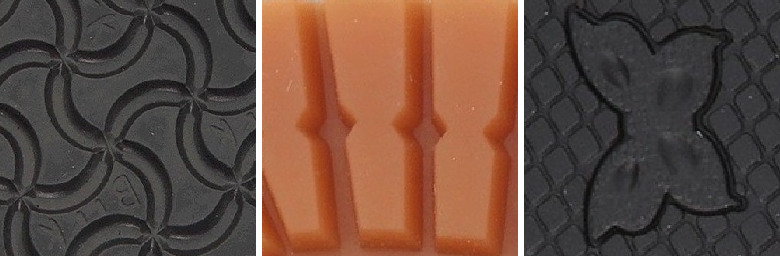
\includegraphics[width=.3\linewidth]{class_examples/bowtie_examples.png}} &
     \raisebox{-.5\height}{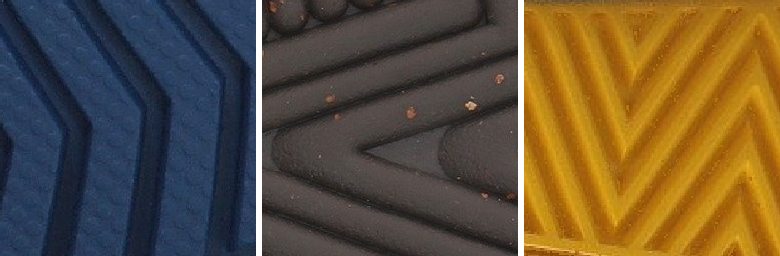
\includegraphics[width=.3\linewidth]{class_examples/chevron_examples.png}} & Chevron \\
     Circle & \raisebox{-.5\height}{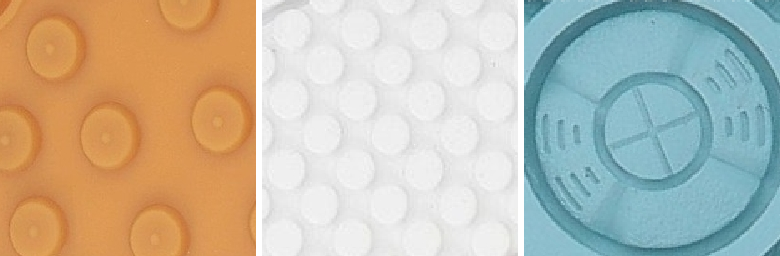
\includegraphics[width=0.3\linewidth]{class_examples/circle_examples.png}} &
     \raisebox{-.5\height}{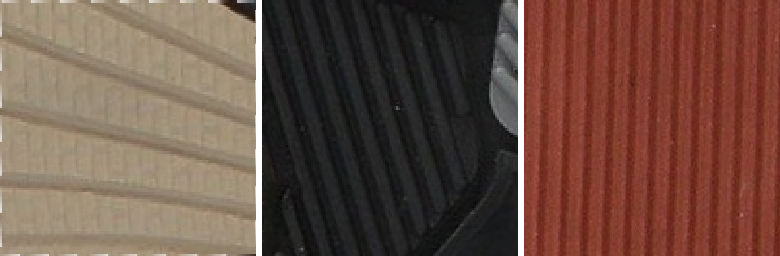
\includegraphics[width=0.3\linewidth]{class_examples/line_examples.png}} & Line \\
     Polygon & \raisebox{-.5\height}{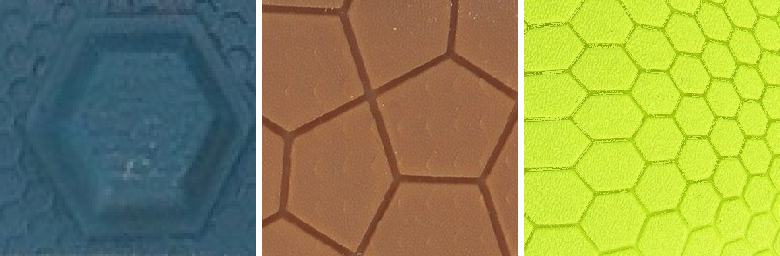
\includegraphics[width=0.3\linewidth]{class_examples/polygon_examples.png}} &
     \raisebox{-.5\height}{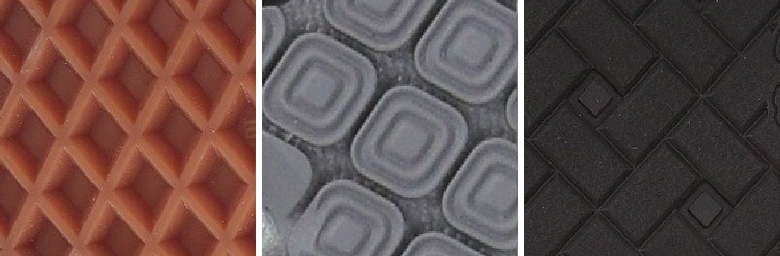
\includegraphics[width=0.3\linewidth]{class_examples/quad_examples.png}} & Quad \\
     Star & \raisebox{-.5\height}{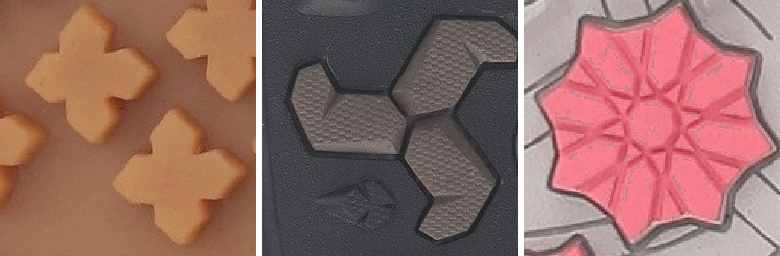
\includegraphics[width=0.3\linewidth]{class_examples/star_examples.png}} &
     \raisebox{-.5\height}{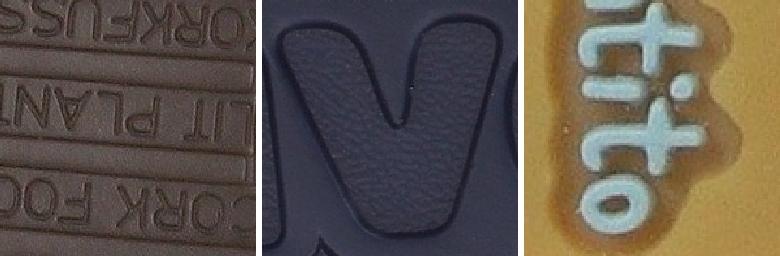
\includegraphics[width=0.3\linewidth]{class_examples/text_examples.png}} & Text \\
     Triangle & \raisebox{-.5\height}{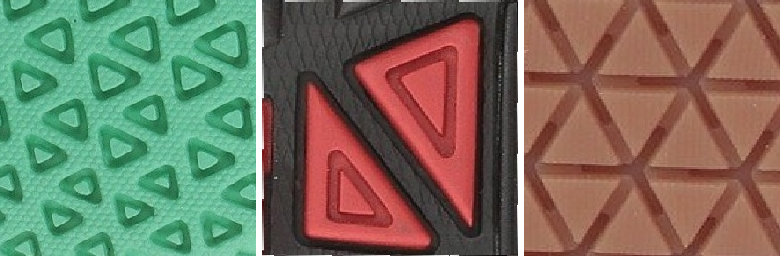
\includegraphics[width=0.3\linewidth]{class_examples/triangle_examples.png}} &
      \raisebox{-.5\height}{} & \\
\end{tabu}
\label{tab:classchars}
\captionof{table}{Geometric shapes, modified from \cite{grossVariabilitySignificanceClass2013}}
\end{minipage}

An automated algorithm which can identify these features in shoe images could be used to assemble an open-access database of shoe models searchable by image upload or feature selection. Spatial relationships between geometric features could be added to further reduce the number of shoes with the same characteristics.

}

%----------------------------------------------------------------------------------------
%	CNNs
%----------------------------------------------------------------------------------------

\headerbox{Convolutional Neural Networks}{name=cnn,column=1,row=0,boxpadding=2mm}{ % This block's bottom aligns with the bottom of the poster
\begin{itemize}\compresslist
    \item A convolutional neural network (CNN) is a tool for deep learning that is well-suited to image analysis.
    \item Inspired by the brain, CNNs learn global patterns using a hierarchy of local feature detection and pooling
    \item VGG16 is a CNN \cite{vgg16} pre-trained on $\sim$1.3 million images spanning 1,000 categories from ImageNet \cite{ILSVRC15}.
\end{itemize}

\begin{center}
\hfill\mbox{\tiny{Image source: \url{https://bit.ly/2AmjF6K}}}
\vspace{-24pt}
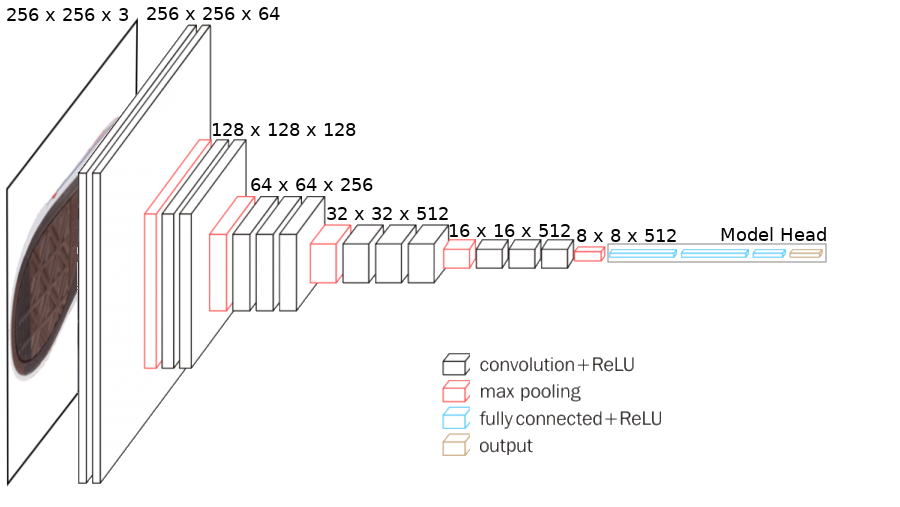
\includegraphics[width=0.9\linewidth]{vgg16-shoe-nolabel.png}
\vspace{2em}
\captionof{figure}{Architecture of VGG16}
\end{center}
\vspace{3pt}
}

%----------------------------------------------------------------------------------------
%	DATA STRUCTURE
%----------------------------------------------------------------------------------------

\headerbox{Data}{name=datastructure,column=1,below=cnn,above=bottom,boxpadding=2mm}{
\begin{minipage}[b]{.495\textwidth}
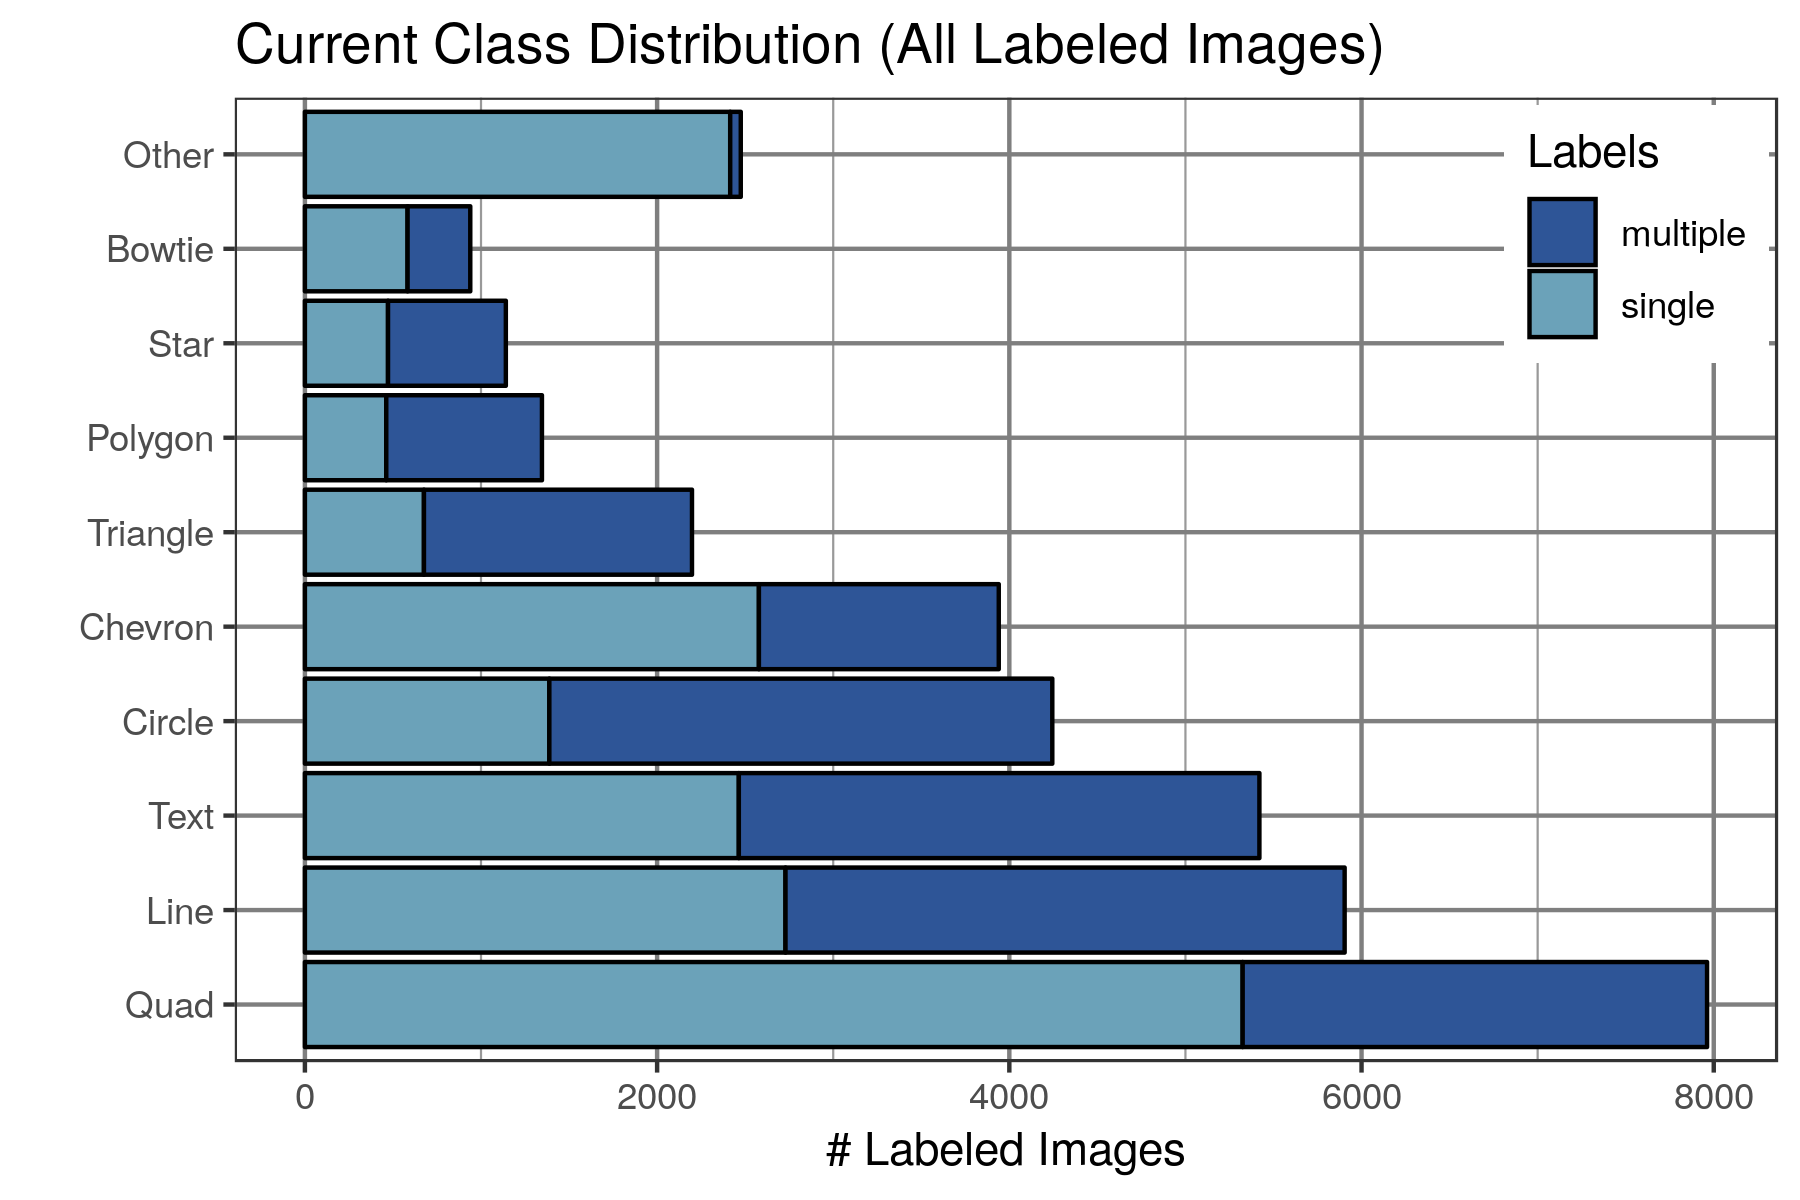
\includegraphics[width=\textwidth]{label-data-barchart-1.png}
\captionof{figure}{Label Frequency}
\end{minipage}\hfill
\begin{minipage}[b]{.495\textwidth}
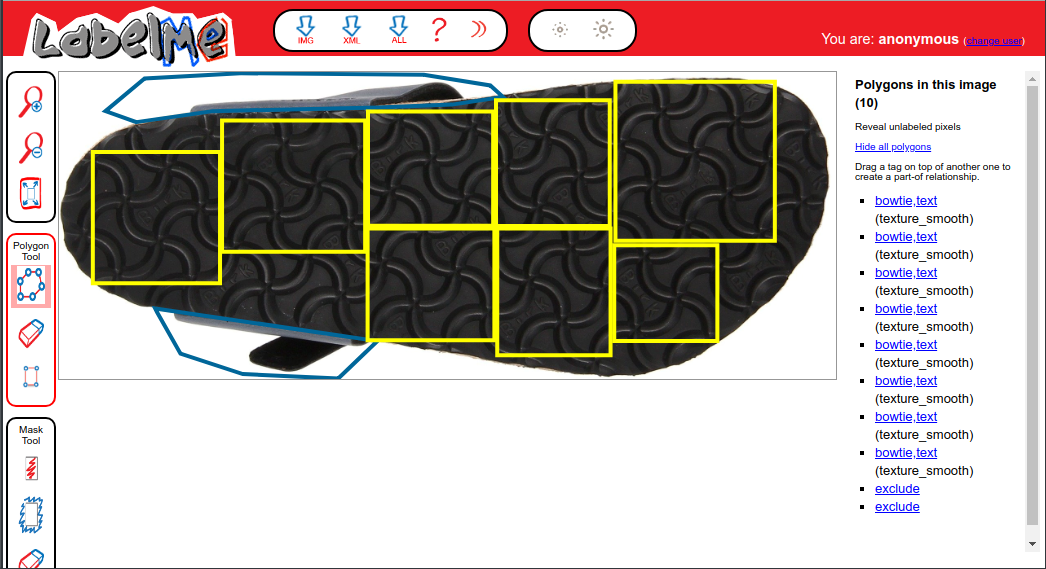
\includegraphics[width=\textwidth]{LabelMeScreenshot.png}
\captionof{figure}{LabelMe Tool \cite{LabelMe}}
\end{minipage}

\vspace{1.35em}
\begin{itemize}
    \item 25,000 multi-label images from 2,200 shoes
    \item Training set: 60\%, downsampled to get approximately equal numbers of each label
    \item Validation set: 20\%, used during training
    \item Test set: 20\%, used after training
\end{itemize}
}

%-------------------------------------------------------------------------------
%	RESULTS 1
%-------------------------------------------------------------------------------


\headerbox{Training}{name=training, column=2, span=1, row=0, boxpadding=2.5mm}{
\begin{center}
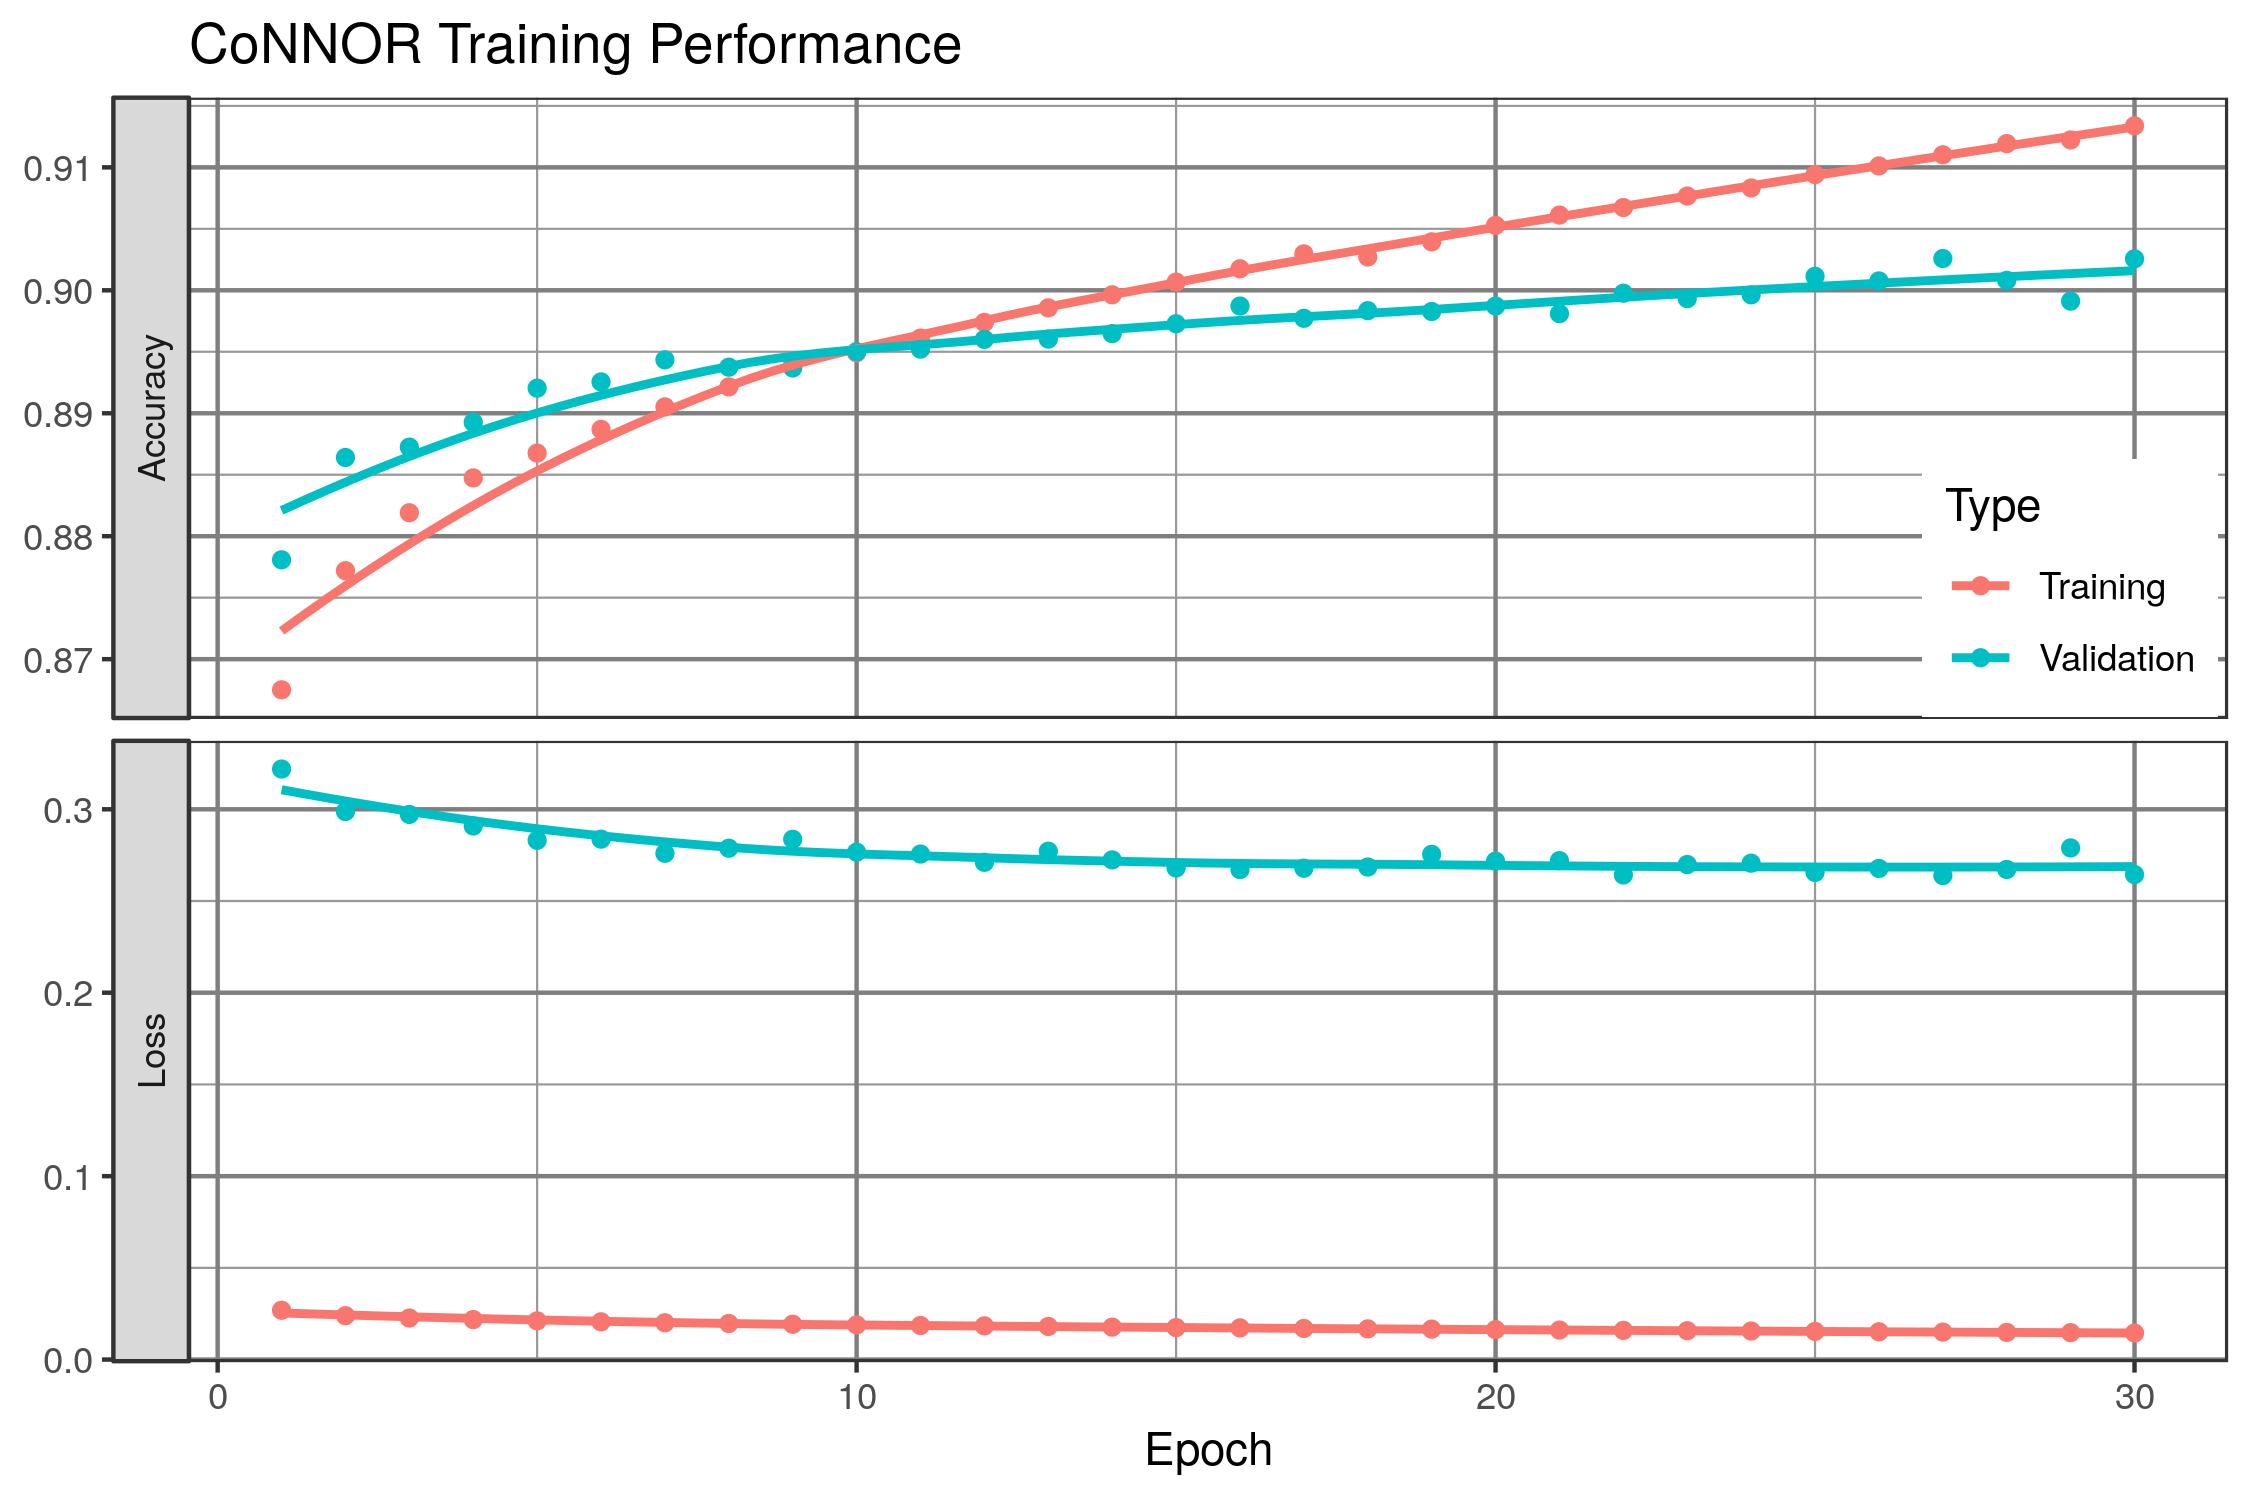
\includegraphics[width=.8\linewidth]{training-accuracy-1.png}
\captionof{figure}{Training and Validation accuracy and loss for each epoch of the fitting process.}
\end{center}
}


\headerbox{Prediction Accuracy}{name=results,column=2,span=1,below=training, above = bottom, boxpadding=2mm}{
%\vspace{1em}
\begin{center}
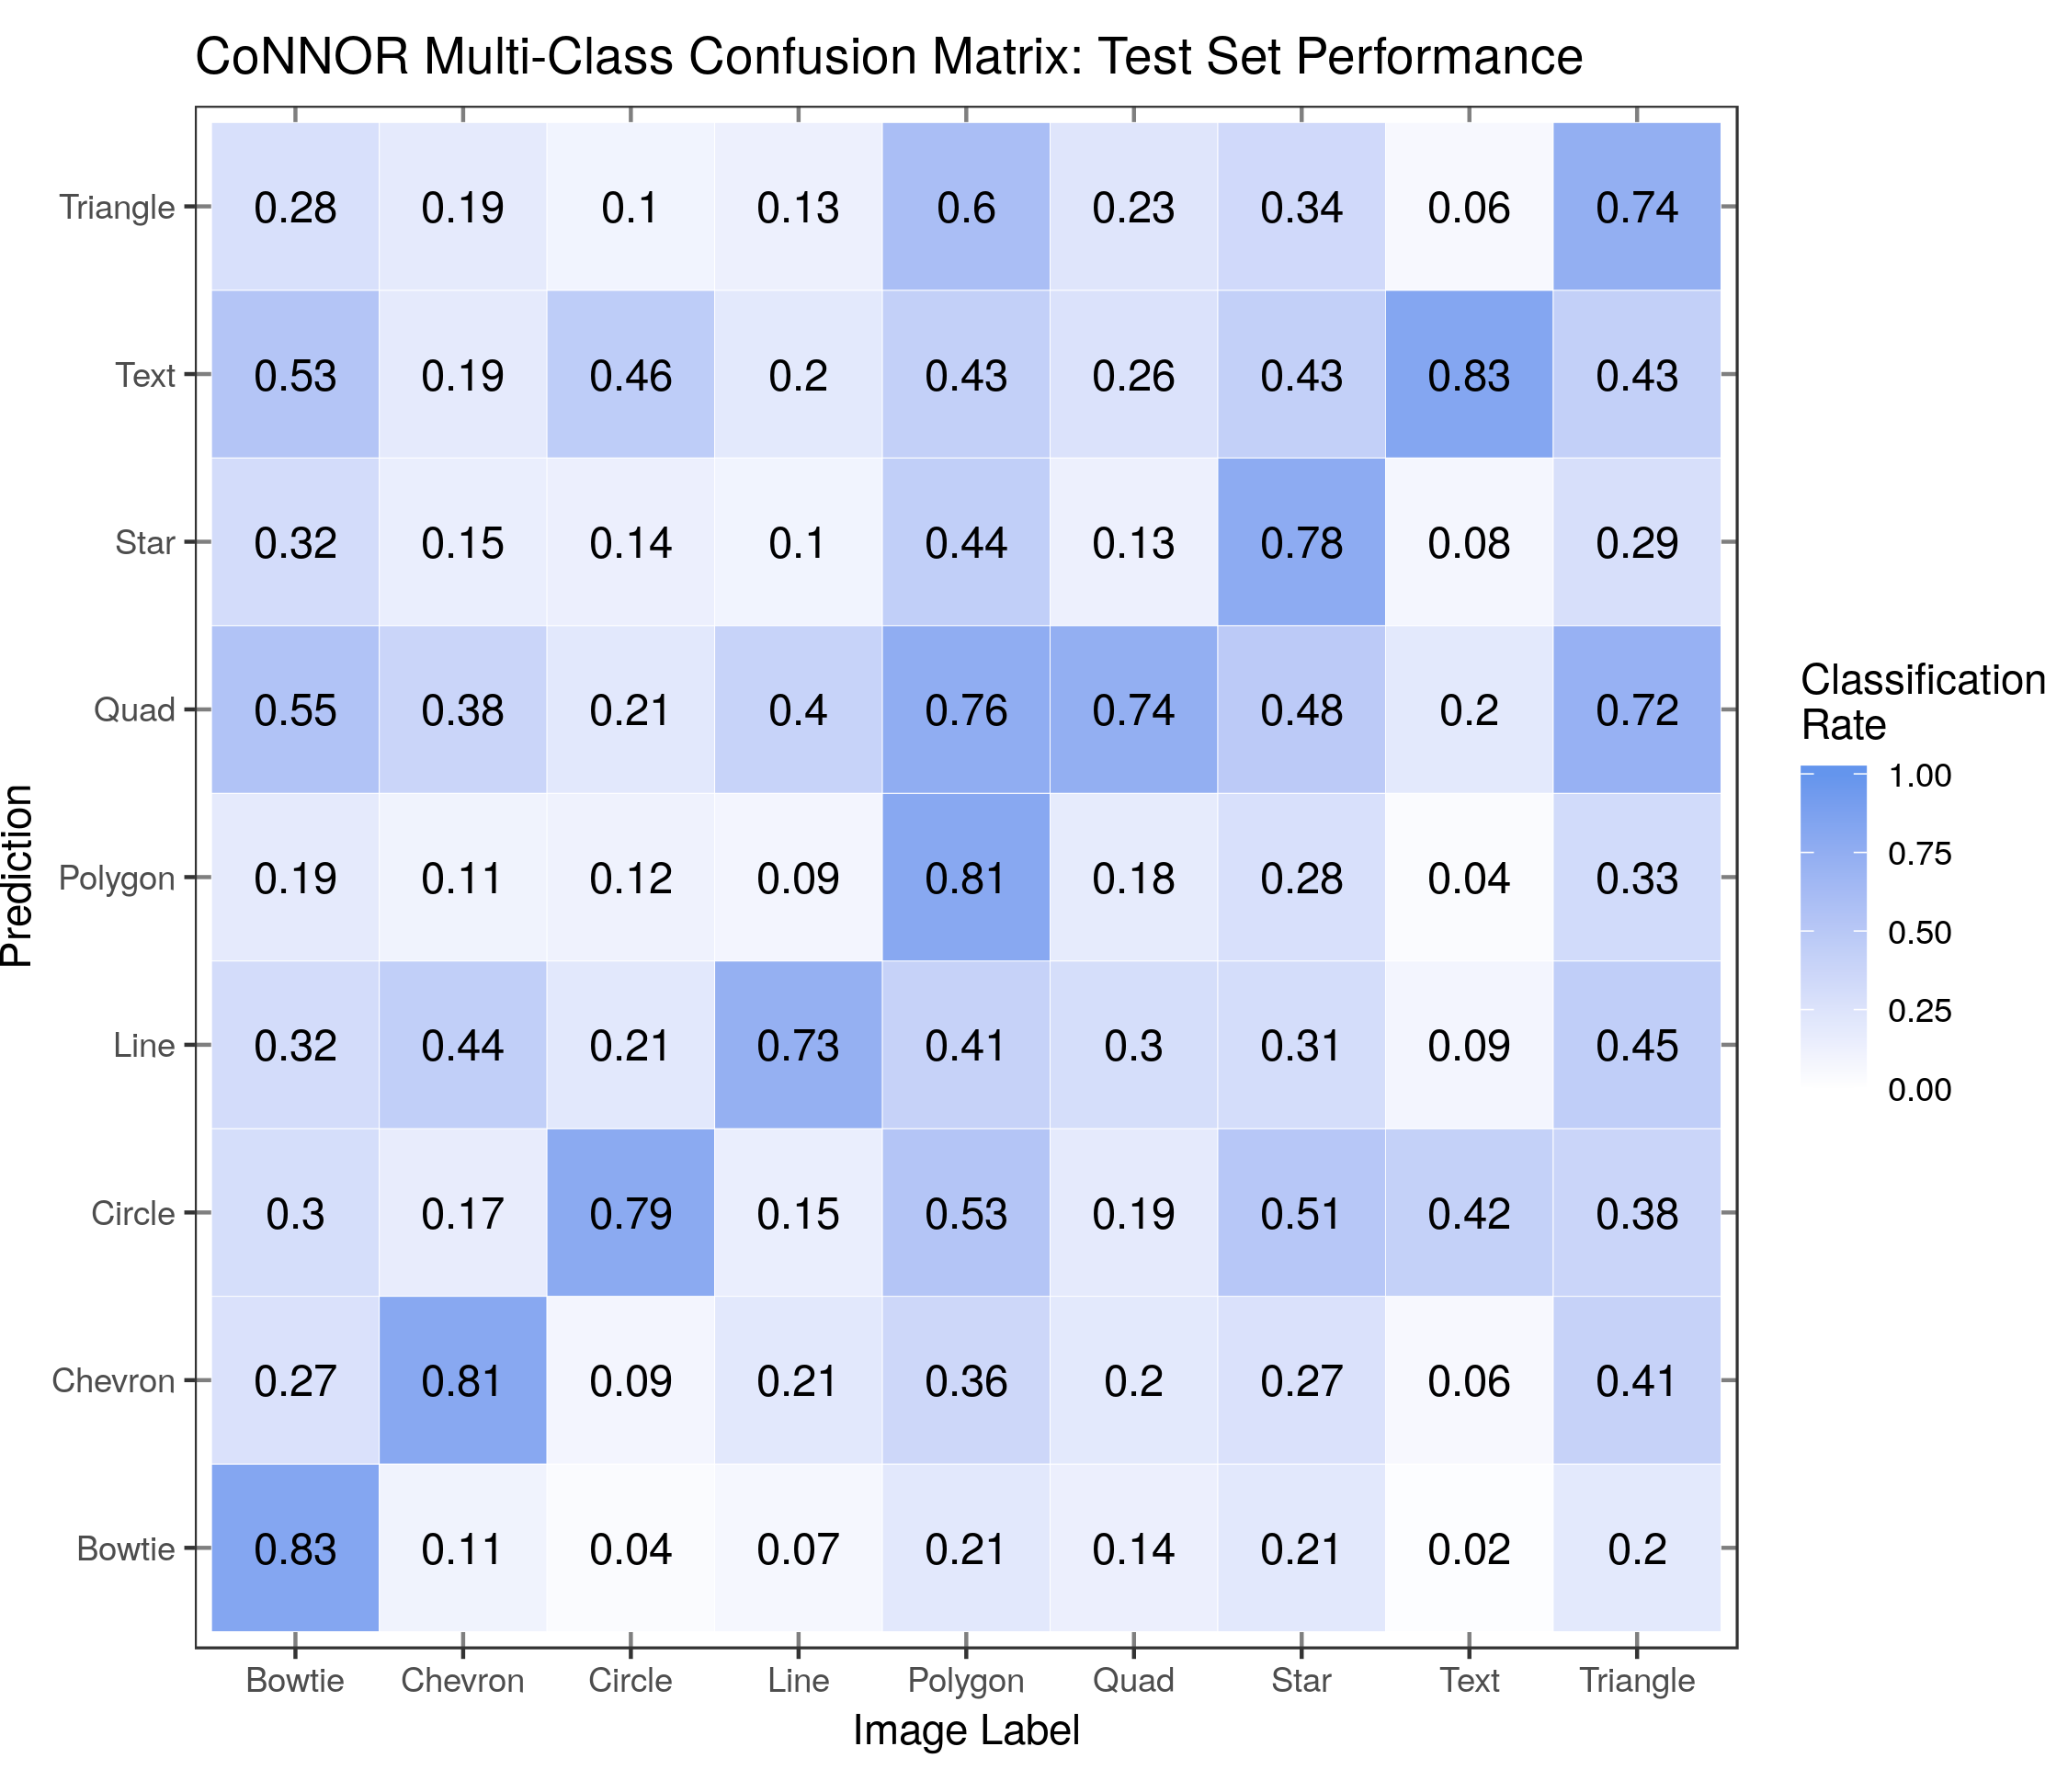
\includegraphics[width=0.68\linewidth]{ConfMatrix-1.png}\hspace{1mm}
\captionof{figure}{Percent of test images identified as containing a class with probability $\geq$ equal error rate, after accounting for multiple labels}

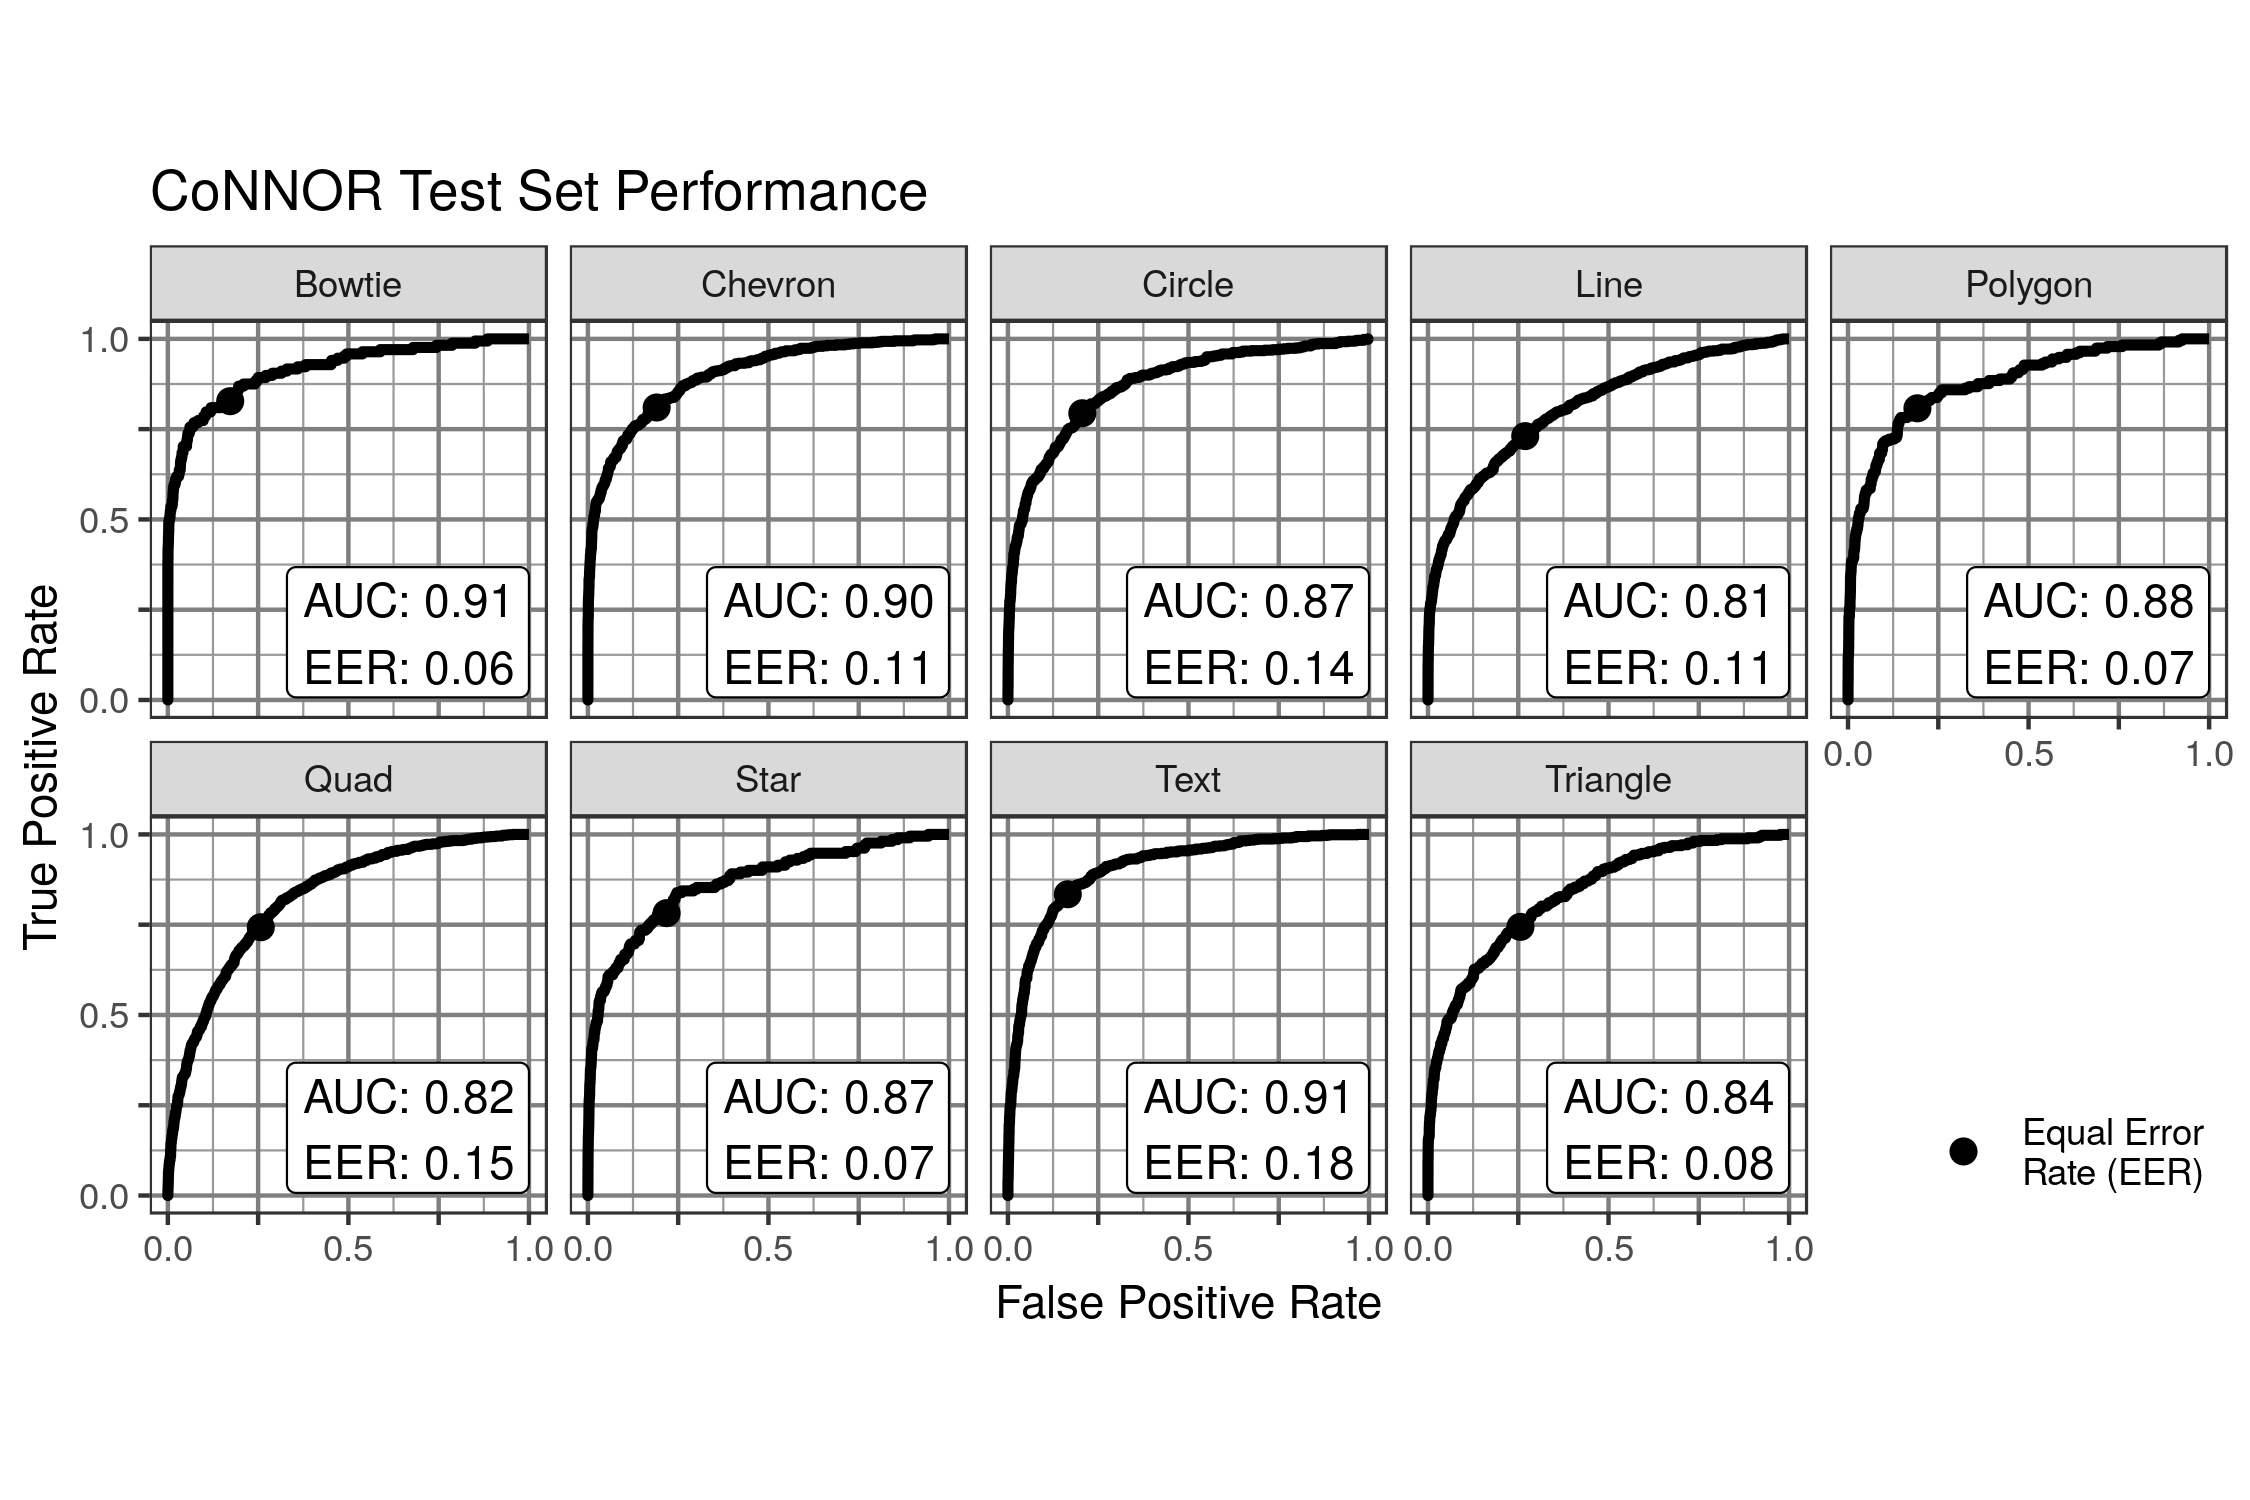
\includegraphics[width=.9\linewidth]{class-roc-1.png}
\captionof{figure}{True Positive Rate by False Positive Rate of classification for each class}
\end{center}
}

\headerbox{Distance}{name=distance, column=3, span=1, row=0, boxpadding=2.5mm}{
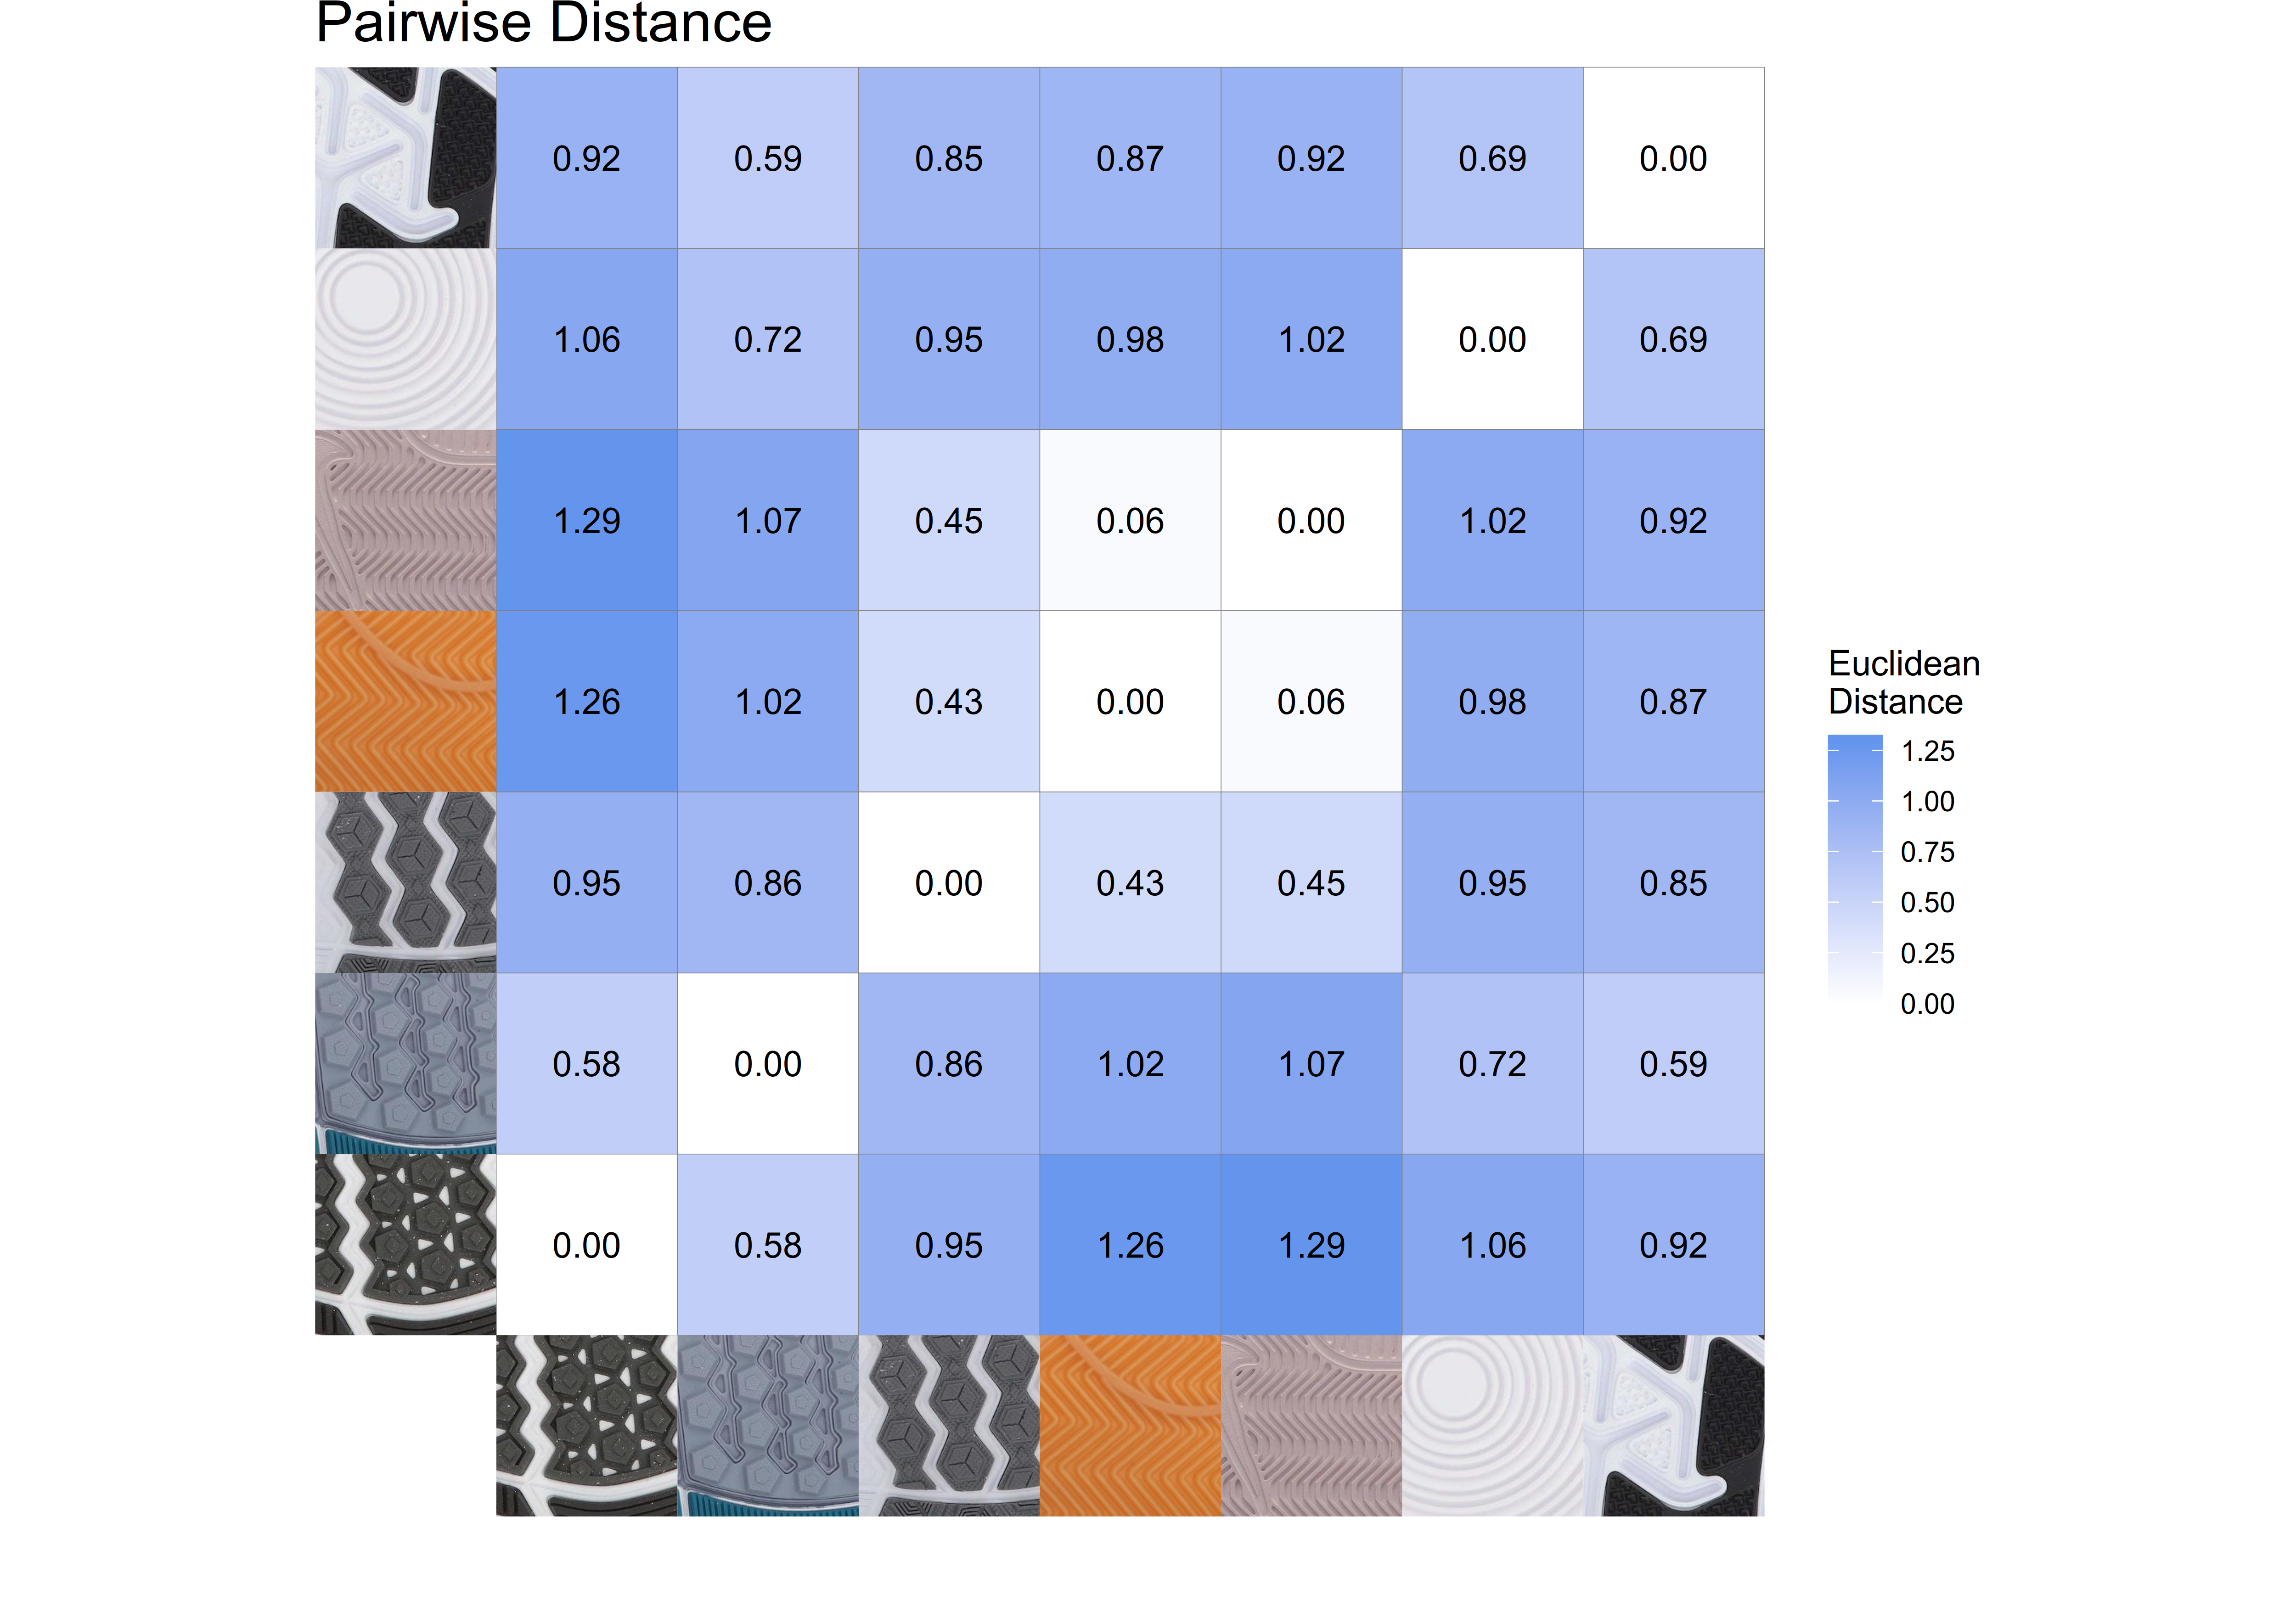
\includegraphics[width=.95\linewidth]{demo-distance-1.png}
\captionof{figure}{Pairwise Euclidean Distance between selected example images}
}


%----------------------------------------------------------------------------------------
%	Applications
%----------------------------------------------------------------------------------------

\headerbox{Future Applications}{name=applications,column=3,span=1,below=distance,boxpadding=2mm}{
\begin{itemize}
    \item Features for statistical models to assess match strength
    \item Speed up database searches
    \item Estimate frequency of class characteristics given information about local population
\end{itemize}
}

%----------------------------------------------------------------------------------------
%	REFERENCES
%----------------------------------------------------------------------------------------

\headerbox{References}{name=references, column=3, span=1, below=applications, above=bottom,boxpadding=2.5mm}{
\renewcommand{\section}[2]{} % Get rid of the default "References" section title
\nocite{*} % Insert publications even if they are not cited in the poster
\scriptsize{ % Reduce the font size in this block
\setlength\bibsep{.35em}
%\begin{multicols}{2}
\raggedright
\bibliographystyle{unsrt}
\bibliography{Refs} % Use sample.bib as the bibliography file
%\end{multicols}
}}





%----------------------------------------------------------------------------------------
% \headerbox{foot}{name=foot,column=0, span=4, above=bottom}{
% abcdefghijklmnop}
%\cfoot{abcdddddddddddd}


\end{poster}
\csafeboilerplate
\end{document}
